% !Mode:: "TeX:UTF-8"
% !TEX program  = xelatex
\documentclass[a4paper]{article}
\usepackage{amsmath}
\usepackage{amssymb}
\usepackage{ctex}
%\usepackage{braket}
%\usepackage[european]{circuitikz}
%\usepackage{multirow}
\usepackage{float}
\usepackage{graphicx}
\usepackage{geometry}
\geometry{left=2.5cm,right=2.5cm,bottom=2.5cm,top=2.5cm}
\title{近代物理实验报告3.2:法拉第效应}
\author{xy\quad 学号\quad 匡亚明学院}
\date{2019年2月29日}
\begin{document}
\maketitle
\bibliographystyle{unsrt}
%--------main-body------------

\section{引言}
1845年,英国科学家法拉第(M. Faraday, 1791$\sim$1867)在探究电磁现象和光学现象之间的关系时发现:当一束平面偏振光穿过介质时,如果在介质中沿光的传播方向加上一个磁场,就会观察到光经过样品后光的振动面转过一个角度,也即磁场使介质具有了旋光性,这种现象后来就称为法拉第效应。

法拉第效应有许多方面的应用,它可以作为物质结构研究的手段,如根据结构不同的碳氢化合物其法拉第效应的表现不同来分析碳氢化合物导体物理的研究中,它可以用来测量载流子得得有效质量、迁移率和提供能带结构的信息;在激光技术中,利用法拉第效应的特性,制成了光波隔离、光频环形器、调制器等;在磁学测量方面,可以利用法拉第效应测量脉冲磁场。

\section{实验目的}
\begin{enumerate}
\item 了解法拉第效应的经典理论。
\item 初步掌握磁光测量的方法。
\end{enumerate}

\section{实验仪器}
\begin{enumerate}
\item 光源系统:白炽灯、透镜组、单色仪、斩光器、起偏器;
\item 磁场系统:电磁铁及供电电源、特斯拉计;
\item 样品介质:可选用费尔得常数大的材料,一般是含重金属或稀土离子的光学玻璃,样品做成柱状;
\item 旋光角检测系统:检偏测角仪、前置放大器、锁相放大器、光电倍增管及其电源和输出指示。
\end{enumerate}

\section{实验原理}
\subsection{法拉第效应}
实验表明,偏振面的磁致偏转可以这样定量描述:当磁场不是很强时,振动面旋转的角度$\theta_F$与光波在介质中走过的路程$l$及磁感应强度在光的传播方向上的分量$B_H$成正比,这个规律又叫法拉第-费尔得定律,即
\begin{equation}
\theta_F = VB_Hl\label{eq1}
\end{equation}
比例系数V由物质和工作的波长决定,表征着物质的磁光特性,这个系数称为费尔得(Verdet)常数,它与光频和温度有关。几乎所有的物质(包括气体液体固体)都有法拉第效应,但是一般都很不显著。不同物质的振动面旋转的方向可能不同。一般规定:旋转方向与产生磁场的螺线管中电流方向一致的,叫正旋(V>0),反之叫负旋(V<0)。

法拉第效应与自然旋光不同。在法拉第效应中,对于给定的物质,偏振面相对于实验室坐标的旋转方向,只由B的方向决定,和光的传播方向无关,这个光学过程是不可逆的。光线往返一周,旋光角将倍增。而自然旋光是可逆的,光线往返一周,累积旋光角为零。与自然旋光类似,法拉第效应也有色散。含有三价稀土离子的玻璃,费尔得常数可以近似表示为
\begin{equation}
V = K(\lambda^2 - \lambda_t^2)^{-1}\label{eq2}
\end{equation}
这里K是透射光波长$\lambda_t$、有效的电偶极矩阵元、温度和浓度等物理量的函数,但是与入射波长$\lambda$无关。这种V值随波长而变得现象称为旋光色散。

做器件用的旋光材料,一般要求有较高的V值、较低的$\alpha$及尽可能小的温度系数。
\subsection{法拉第效应的经典理论}
从光波在介质中传播的图像看,法拉第效应可以这样理解:一束平行于磁场方向传播的平面偏振光,可以看作是两束等幅的的左旋和右旋偏振光的叠加,左旋和右旋是相对于磁场方向而言的。介质中受原子核束缚的电子在入射光的两旋转电矢量作用下,作稳态的圆周运动。在与电子轨道平面相垂直的方向上加一个磁场B,则在电子上将引起径向力$F_M$(即洛伦兹力)可以有两个不同的值。轨道半径也可以由两个不同的值。结果,对于一个给定的磁场就会有两个电偶极矩,两个电极化率。这样,磁场的作用就使左旋圆偏振光的折射率$n_L$和右旋圆偏振光的折射率$n_R$不等,通过厚度为$l$的介质后,将产生不同的位相滞后
\begin{equation}
\phi_R = \frac{2\pi}{\lambda}n_Rl\text{, }\phi_L = \frac{2\pi}{\lambda}n_Ll\label{eq3}
\end{equation}
式(\ref{eq3})中的$\lambda$是真空中的波长。
\begin{figure}[!h]
\centering
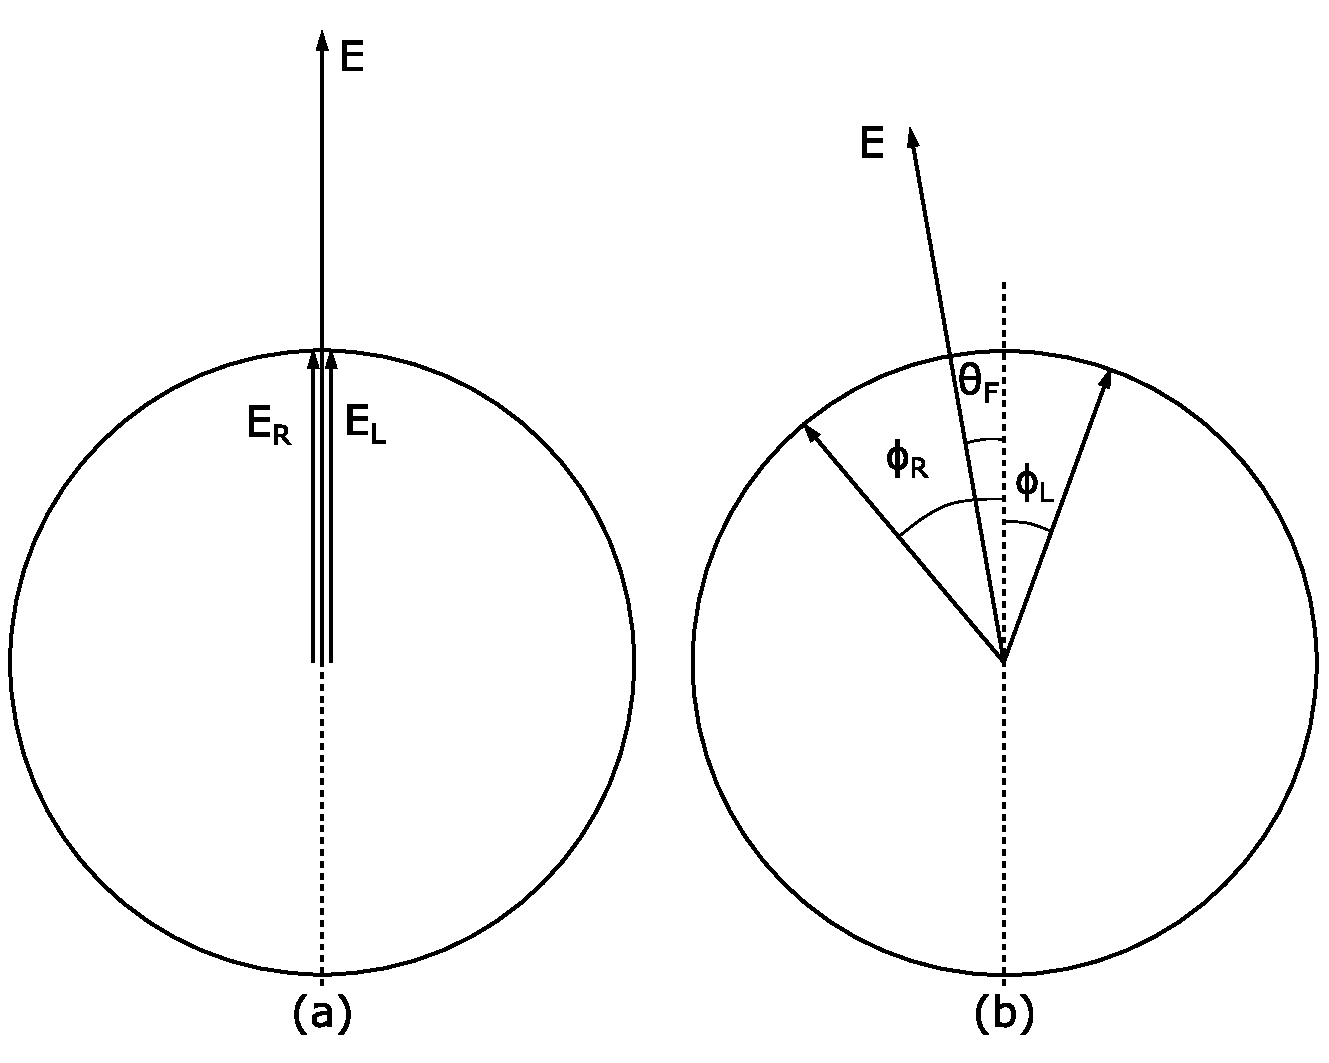
\includegraphics[width=0.6\textwidth]{fig/fig3.pdf}
\caption{旋光的解释}\label{fig3}
\end{figure}

圆偏振光的相位即旋转矢量的角位移,相位滞后即角位移的倒转。在介质的入射面上,入射的平面偏振光E可以分解为如图(\ref{fig3}-a)所示的两个旋转方向不同的圆偏振光$E_L$和$E_R$。通过介质后,它们的相位滞后旋转矢量如图(\ref{fig3}-b)所示,从介质出射后,两个圆偏振光的合成矢量E的方向相对于原来的方向转过的角度是
\begin{equation}
\theta_F = \frac{1}{2}(\phi_R - \phi_L) = \frac{\pi}{\lambda}(n_R - n_L)l\label{eq4}
\end{equation}
假如和的差正比于磁感应强度B,由式(\ref{eq4})可以得到式(\ref{eq1})。
磁场使左右旋圆偏振光的折射率不同,从微观上理解:这在本质上可以归结为在磁场的作用下原子、分子能及和量子态的变化。法拉第效应的严格推导涉及到色散的量子力学理论。
\subsection{法拉第旋光角的计算}
设介质中原子的轨道电子具有磁矩$\mathbf{\mu}$:
\begin{equation}
\mathbf{\mu} = -\frac{2}{2m_e}\mathbf{L}\label{eq5}
\end{equation}
式中$\mathbf{L}$是轨道角动量。在磁场B中,一个电子磁矩具有势能$E_p$为
\begin{equation}
E_p = -\mathbf{\mu}\cdot\mathbf{B} = \frac{e}{2m_e}\mathbf{L}\cdot\mathbf{B} = \frac{eB}{2m_e}L_{\text{轴}}\label{eq6}
\end{equation}
式中$L_{\text{轴}}$为电子轨道角动量的轴向分量。
当平面偏振光通过磁场B作用在折射率为n的样品介质上,光子使电子由基态激发到高能态。处于激发态的电子吸收光子的角动量$\pm h$,动能没有改变,而势能则增加$\Delta E_p$
\begin{equation}
\Delta E_p = \frac{eB}{2m_e}\Delta E_{p\text{轴}} = \pm\frac{eB}{2m_e}L_{\text{轴}}\label{eq7}
\end{equation}
同时光子失去能量$\Delta E_p$。式(\ref{eq7})中的正负号对应于左旋光和右旋光。

因为光子具有能量$h\nu$,故样品介质对光的折射率n是$\hbar\omega$的函数:
\begin{equation}
n = n(\hbar\omega)\label{eq8}
\end{equation}
对左旋光量子来说,
\begin{equation*}
n_L = n(\hbar\omega - \Delta E_p^{'})
\end{equation*}
或
\begin{equation}
n_L = n\left(\omega - \frac{\Delta E_p^{'}}{\hbar}\right)\approx n(\omega) - \frac{\text{d}n}{\text{d}\omega}\frac{\Delta E_p^{'}}{\hbar} = n(\omega) - \frac{eB}{2m_e}\frac{\text{d}n}{\text{d}\omega}\label{eq9}
\end{equation}
同理,对右旋光量子有
\begin{equation}
n_R = n(\omega)+\frac{eB}{2m_e}\frac{\text{d}n}{\text{d}\omega}\label{eq10}
\end{equation}
把式(\ref{eq9})、(\ref{eq10})带入式(\ref{eq4})得
\begin{equation}
\theta_F = \frac{lBe}{2m_ec}\omega\frac{\text{d}n}{\text{d}\omega}\label{eq11}
\end{equation}
用波长表示,得
\begin{equation}
\theta_F = -\frac{lbe}{2m_ec}\lambda\frac{\text{d}n}{\text{d}\lambda}\label{eq12}
\end{equation}
这是法拉第效应旋光角的计算公式。它表明旋光角的大小和样品介质的厚度、磁感应强度成正比,和入射光的波长及样品介质的色散$\frac{\text{d}n}{\text{d}\lambda}$有密切关系。

\section{实验内容}
\begin{enumerate}
\item 确定磁场及光电倍增光的旋钮处于逆时针的最小位置,打开电源。
\item 磁场调零。
\item 光电倍增管电压换换调至850V(\CJKunderdot{必须}<1000V),调节过程中注意输出指示不可以过载。
\item \CJKunderdot{缓慢转动}检偏调节旋钮寻找消光点,这就是法拉第转角的零点。
\item 固定光的波长为500nm,不断增大磁场值(必须$\leq$600mT),分别在0, 100, 200, 300, 400, 500, 600mT处测量检偏角,算出Faraday转角。
\item 再分别取波长为550nm, 633nm, 700nm(沿一个方向\CJKunderdot{缓慢转动}波长调节旋钮),分别在0, 200, 400, 600mT处测量检偏角,算出Faraday转角。
\item 换一个样品重做步骤5和6。
\item (选作)固定磁场值为500mT,在400nm$\sim$700nm范围内间隔50nm改变光的波长(沿一个方向\CJKunderdot{缓慢转动}波长调节旋钮),分别测量检偏角,取步骤5或6中0T处的检偏角值为零点,计算Faraday转角、费尔得常数。
\end{enumerate}

\section{注意事项}
\begin{enumerate}
\item 先把磁场调零,光电倍增管的负电压调至绝对值小于300V ,然后再开电源、关电源以及换样品。
\item 磁场处于最大值(600mT)的时间不能太长,否则仪器发热容易损坏。
\item 尽量沿一个方向缓慢转动波长调节旋钮、检偏调节旋钮。
\end{enumerate}

\section{实验数据}

\section{误差分析}
\iffalse
\begin{enumerate}
\item 消光法测量时光电流反应不够灵敏,最小值不够准确,导致对应的检偏器角度读取有误差。
\item 光路不满足实验要求,精度不够导致测量不准确。
\item 读数有一定误差。综合导致测量点不再一条直线上。
\end{enumerate}
\fi

\section{思考题}
\subsection{材料的法拉第效应的大小与哪些因素有关?}
\subsection{简述本实验测定法拉第转角所采用的试验方法?}
\subsection{本实验的法拉第效应和透明磁性材料的法拉第效应有何异同?}
\subsection{有些材料除了有法拉第旋光效应以外,还有自然旋光,双折射现象,它们会影响本实验测量的准确度,用什么方法可以消除这些因素的影响?}

\nocite{jiaocai}
\bibliography{ref}
\end{document}